\documentclass[12pt]{article}
\usepackage[portuguese]{babel}
\usepackage{natbib}
\usepackage[export]{adjustbox}
\usepackage{float}
\usepackage{url}
\usepackage[utf8x]{inputenc}
\usepackage{mathtools}  
\usepackage{graphicx}
\graphicspath{images}
\usepackage{listings}
\usepackage[margin=2cm]{geometry}
\usepackage{wrapfig}
\renewcommand*{\thesubsubsection}{\alph{subsubsection}.}
\usepackage{multicol}
\usepackage{caption}

\begin{document}

\begin{titlepage}

\center % Center everything on the page

\newcommand{\HRule}{\rule{\linewidth}{0.4mm}} % Barra horizontal

\textsc{\LARGE Universidade do Minho}\\[0.5cm]  % Name of your university/college

\vspace{1cm}
\textsc{\large Licenciatura em Engenharia Informática}\\[1.5cm] % Nome do curso
\vspace{0.5cm}

\HRule \\[0.5cm]
{ \LARGE \bfseries } Redes de Computadores \\[0.5cm] % Título
{ \LARGE \bfseries } \textbf{Grupo 135} \\[0.5cm] % Grupo
\HRule \\[1cm]
\vspace{0.1cm}
 
\paragraph{}
\paragraph{}
\textsc{\Large \textbf{TP2: Protocolo IPv4 }}\\[0.75cm] % Nome da UC
\vspace{2.5cm} % Autores
Joana Alves (A93290) \\ \vspace{3mm}
João Machado (A89510) \\ \vspace{3mm} 
Rui Armada (A90468) \\ \vspace{3mm}

\vspace{3cm}


\vspace*{\fill}

{\large Abril 2022}\\[2cm] % Data

\vfill % Fill the rest of the page with whitespace
\end{titlepage}




% ----- PARTE I -------
\section*{\hfil Parte I\hfil}
\section{Questões e Respostas}
\subsection{Questão 1 - Topologia Core}
De acordo com as instruções presentes no enunciado, apresentamos de seguida 
a topologia construída, tendo em conta a alteração do tempo de propagação para
10 ms:

\paragraph{}
\begin{figure}[H]
\centering
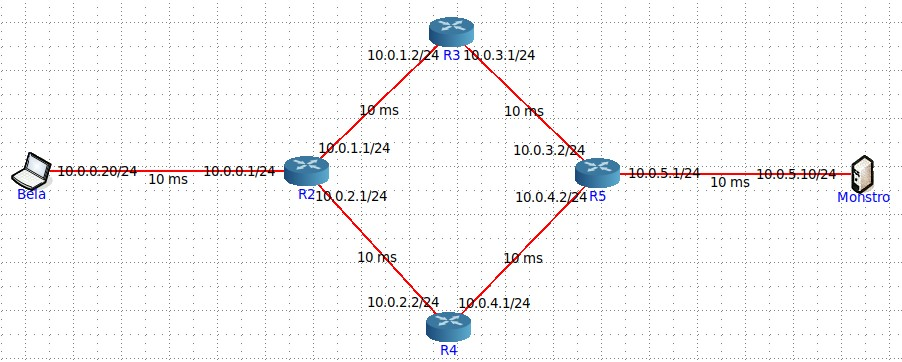
\includegraphics[width=500pt]{images/ParteI/Questao1/questao1-topologia.jpg}
\caption{Topologia (Questão 1).} \label{topologia}
\end{figure}


\paragraph{}
\subsubsection{Active o \textit{wireshark} ou o \textit{tcpdump} no \textit{host} Bela. Numa \textit{shell} de Bela execute o comando \textit{traceroute -I} para o endereço IP do Monstro}

\begin{figure}[H]
\centering
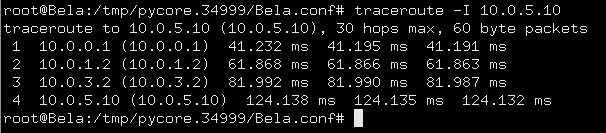
\includegraphics[width=400pt]{images/ParteI/Questao1/questao1-a.jpg}
\caption{Print da \textit{shell} no \textit{host} Bela.} \label{questao1-a}
\end{figure}

%
%
\subsubsection{Registe e analise o tráfego ICMP enviado pelo sistema Bela e o tráfego ICMP recebido como resposta. Comente os resultados face ao comportamento esperado.}



\begin{figure}[H]
\centering
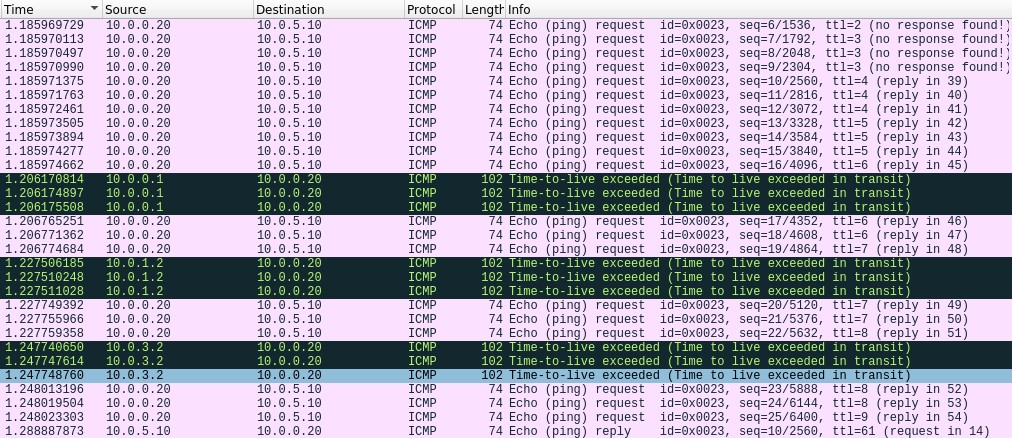
\includegraphics[width=\linewidth]{images/ParteI/Questao1/questao1-wireshark.jpg}
\caption{Tráfego ICMP enviado e recebido pelo \textit{host} Bela.} \label{1-wireshark}
\end{figure}

    O comando \textit{traceroute} envia, através do \textit{host}, vários datagramas ICMP variando o valor de TTL (\textit{Time To Live}) para assim obter a rota desde a origem até ao IP destino (especificado no comando \textit{traceroute}). A variável TTL indica o número de saltos que o datagrama pode fazer dentro da rede antes de ser considerado inválido, sendo este valor decrementado sempre que executa um salto. O seu comportamento, de forma resumida, pode ser descrito como o envio sequencial de conjuntos de um ou mais datagramas ICMP com o mesmo TTL, iniciando este valor a 1 e incrementando a cada iteração. Um \textit{host} ao verificar que o valor do TTL de um datagrama é 0 envia como resposta uma mensagem de controlo (datagrama ICMP) com a informação de 'TTL \textit{exceeded}'. Assim, o \textit{host} que enviou os datagramas iniciais vai obtendo, ao longo das iterações, uma noção cada vez mais completa da rota até ao destino.
    
    \par No caso concreto deste exercício, podemos, através da Figura \ref{1-wireshark}, verificar o envio destes conjuntos de três datagramas ICMP logo a partir da primeira linha, começando, tal como dito, no valor TTL=1 e sendo incrementado a cada iteração.
    
    \par Apresentamos, de seguida, uma tabela com a correspondência entre os valores iniciais de TTL dos datagramas e os \textit{hosts} que os receberam quando estes atingiram o valor 0, ou seja, excederam o seu número de saltos na rede: 
    
        \begin{wrapfigure}{r}{0.25\textwidth}
        \begin{center}
        \vspace{-20pt}
            \begin{tabular}{|c|c|}
            \cline{1-2}
            TTL & Host Final  \\
            \hline \hline
             1 & 10.0.0.1 \\
             2 & 10.0.1.2 \\
             3 & 10.0.3.2 \\
            \cline{1-2}
        \end{tabular}
        \end{center}
    \end{wrapfigure}
        
    \par Como podemos verificar pela tabela, os datagramas enviados com TTL=1 ficaram inválidos no \textit{host} 10.0.0.1, os datagramas com TTL=2 no \textit{host} 10.0.1.2 e, por fim, os datagramas com TTL=3 foram invalidados pelo \textit{host} 10.0.3.2. 
    
    \par Podemos reparar que os datagramas com TTL superior a 3 não registaram nenhuma resposta de 'TTL \textit{exceeded}' uma vez que a partir desse valor os pacotes conseguem chegar a qualquer nodo da rede, inclusive o nodo objetivo (10.0.5.10).
    
\subsubsection{Qual deve ser o valor inicial mínimo do campo TTL para alcançar o servidor \textit{Monstro}? Verifique na prática que a sua resposta está correta.}
    
    \par O valor mínimo do campo TTL necessário para alcançar o servidor \textit{Monstro} será \textbf{4}, uma vez que valores inferiores a 3 (inclusive) têm resposta de tempo de vida excedido (como visto na alínea anterior). Podemos verificar isto pela não receção de datagramas ICMP por parte do \textit{host} Bela a partir dos valores de TTL superiores ou iguais a 4, ou pelo cálculo direto através da observação da topologia, onde verificamos que são necessários, no mínimo, quatro saltos para atingir o servidor.



\subsubsection{Calcule o valor médio do tempo de ida-e-volta (RTT - \textit{Round-Trip Time}) obtido no acesso ao servidor. Para melhorar a média, poderá alterar o número pacotes de prova com a opção -q.}

    \begin{figure}[H]
        \centering
        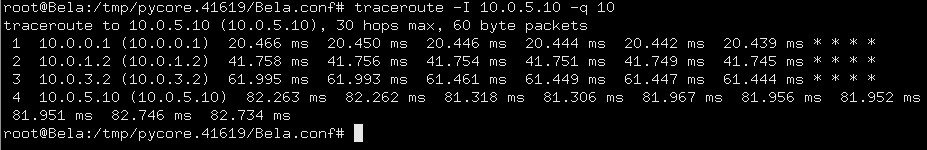
\includegraphics[width=500pt]{images/ParteI/Questao1/questao1-d.jpg}
        \caption{Aplicação do comando 'traceroute -I 10.0.5.10 -q 10'.} \label{tracerouteMedia}
    \end{figure}
    
    \par De acordo com o resultado do comando pedido, retiramos os valores atingidos no acesso ao servidor \textit{Monstro} a partir da linha numerada com o valor 4. Assim, calculamos a média destes mesmos valores, tendo obtido o seguinte resultado:

    \begin{align*}  
    \frac{82.263+82.262+81.318+81.306+81.967+81.956+81.952+81.951+82.746+82.734}{10} = 81.946 ms  
    \end{align*}  
    


\subsubsection{O valor médio do atraso num sentido (One-Way Delay) poderia ser calculado com precisão dividindo o RTT por dois? O que torna difícil o cálculo desta métrica?}
    
    O cálculo torna-se difícil devido às exigências de sincronização, uma vez que \textit{delay} é uma métrica que exige sincronização de relógios. \textit{One-Way Delay}, tal como o nome indica, só funciona num sentido, mas precisa de ter acesso a algumas informações para poder ser calculado, nomeadamente o registo de quando o pacote foi enviado (\textit{timestamp}). Em consequência, é imperativo que os relógios estejam sincronizados, caso contrário esta informação torna-se irrelevante.
     O \textit{delay} de ida é diferente do de volta pois o percurso percorrido pode não ser idêntico, por conseguinte, o valor médio de atraso num sentido não pode ser calculado com precisão dividindo o RTT por dois.
    
    

\newpage
% -------------------------- QUESTÃO 2 ------------------------------
\subsection{Questão 2 - \textit{Traceroute}}

 \begin{figure}[H]
 \centering
 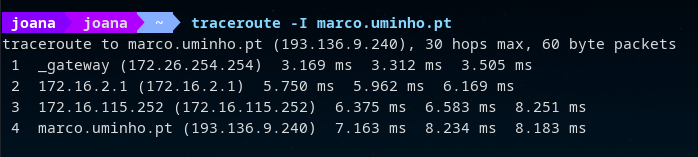
\includegraphics[width=400pt]{images/ParteI/Questao2/questao2-comando.png}
 \caption{Resultado do comando \textit{traceroute} na máquina nativa.} \label{questao2-comando}
 \end{figure}
    
 \begin{figure}[H]
 \centering
 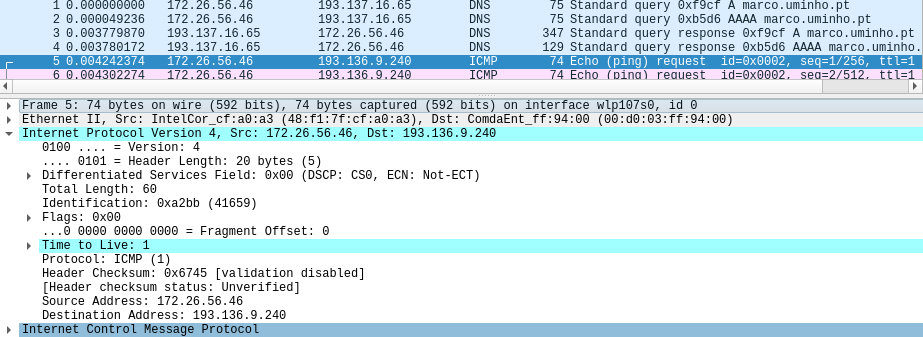
\includegraphics[width=500pt]{images/ParteI/Questao2/questao2-a)primeiroPacote.png}
 \caption{Informação da primeira mensagem ICMP enviada pela máquina.} \label{questao2-IPMaquinaNativa}
 \end{figure}
 

\subsubsection{Qual é o endereço IP da interface ativa do seu computador?}

    \par Como se pode observar na Figura \ref{questao2-IPMaquinaNativa}, na informação da mensagem ICMP enviada pela máquina nativa, no parâmetro \textit{Source Address}, a interface que foi utilizada para realizar este teste possui o endereço IP de \textbf{172.26.56.46}.


\subsubsection{Qual é o valor do campo protocolo? O que permite identificar?}

    \par Como podemos verificar pela Figura \ref{questao2-IPMaquinaNativa}, o valor do campo \textit{Protocol} é 1, correspondendo ao protocolo ICMP. O conteúdo deste campo especifica o protocolo que está a ser encapsulado pelo IP para assim permitir a descodificação do mesmo pelas camadas devidas. 



\subsubsection{Quantos bytes tem o cabeçalho IPv4? Quantos bytes tem o campo de dados (payload) do datagrama? Como se calcula o tamanho do payload?}

    \par O cabeçalho IPv4 tem um total de 20 \textit{bytes}. Uma vez que o \textit{payload} se calcula subtraindo o tamanho do cabeçalho ao tamanho total do datagrama, o campo de dados tem 40 (60-20) \textit{bytes}.


\subsubsection{O datagrama IP foi fragmentado? Justifique.}

    \par O datagrama não foi fragmentado uma vez que a \textit{flag} de não fragmentação não está definida no cabeçalho no campo \textit{Flag}. Para além disso, podemos verificar que o valor do \textit{offset} é 0, logo estamos perante o datagrama original, sem fragmentação.



\subsubsection{Ordene os pacotes capturados de acordo com o endereço IP fonte (e.g., selecionando o cabeçalho da coluna Source), e analise a sequência de tráfego ICMP gerado a partir do endereço IP atribuído à interface da sua máquina. Para a sequência de mensagens ICMP enviadas pelo seu computador, indique que campos do cabeçalho IP variam de pacote para pacote.}

    \begin{figure}[H]
    \centering
    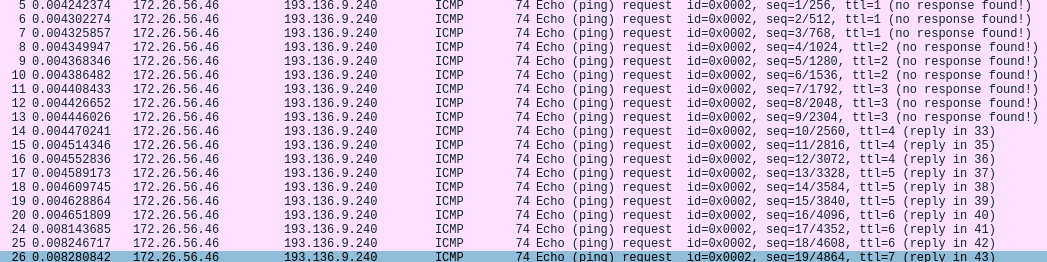
\includegraphics[width=500pt]{images/ParteI/Questao2/questao2-ICMPdaMaquina.png}
    \caption{Sequência de mensagens ICMP enviadas pela máquina.} \label{questao2-SequenciaICMP-1}
    \end{figure}

    \begin{minipage}{0.5\linewidth}
    \centering
        \begin{figure}[H]
        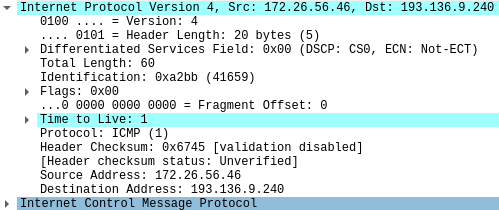
\includegraphics[width=0.95\linewidth]{images/ParteI/Questao2/questao2-PrimeiroPacoteCabecalho.png}
        \caption{Primeiro pacote com TTL=1.} \label{questao2-primeiroPacote}
        \end{figure}
    \end{minipage}
    \begin{minipage}{0.5\linewidth}
    \centering
        \begin{figure}[H]
        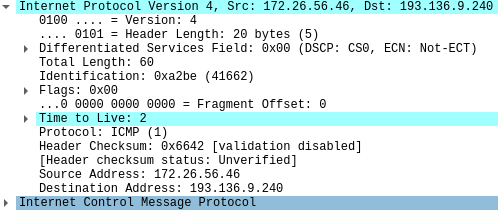
\includegraphics[width=0.95\linewidth]{images/ParteI/Questao2/questao2-primeiro2TTLCabecalho.png}
        \caption{Primeiro pacote com TTL=2.} \label{questao2-SegundoPacote}
        \end{figure}
    \end{minipage}

    \paragraph{}
    \paragraph{}
    \par Analisando os pacotes da sequência de mensagens ICMP enviadas pela máquina nativa, podemos inferir que alguns campos se alteram ao longo da sequência. Assim, conseguimos distinguir os seguintes campos: \textbf{\textit{Identification}, \textit{Checksum}} e \textbf{TTL}. O \textit{checksum} é um parâmetro de controlo de integridade do pacote, sendo, por isso, normal que o seu valor não coincida. Relativamente aos outros dois campos, é explicado na alínea seguinte.
    

\newpage
\subsubsection{Observa algum padrão nos valores do campo de Identificação do datagrama IP e TTL?}

    \par O campo de identificação é incrementado sequencialmente e o campo TTL vai incrementando em conjuntos de trẽs pacotes, ou seja, três pacotes são enviados com o mesmo valor (TTL = k) seguidos de outros três com o valor inteiro diretamente acima (TTL = k+1).
 

\subsubsection{Ordene o tráfego capturado por endereço destino e encontre a série de respostas ICMP TTL \textit{exceeded} enviadas ao seu computador. Qual é o valor do campo TTL? Esse valor permanece constante para todas as mensagens de resposta ICMP TTL \textit{exceeded} enviados ao seu \textit{host}? Porquê?}

    \begin{figure}[H]
    \centering
    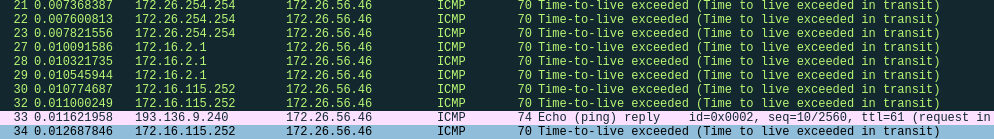
\includegraphics[width=500pt]{images/ParteI/Questao2/questao2-TTLExceeded.png}
    \caption{Sequência de mensagens ICMP enviadas pelo endereço destino.} \label{questao2-SequenciaICMP-2}
    \end{figure}
    
    \par O campo TTL não se mantém constante para todas as mensagens de resposta, tendo um valor diferente para cada \textit{host}. Isto acontece porque como os pacotes são enviados pelos \textit{routers} em que o TTL falha, o número de saltos necessários para atingir a nossa máquina ou definidos como \textit{default} pelos mesmos variam.
    
    
    
\newpage
% --------------------- QUESTÃO 3 ------------------------------
\subsection{Questão 3 - Fragmentação}

    \par De acordo com o requisito do enunciado, executamos o comando \textit{traceroute} definindo o tamanho do pacote para 4000 + 135 (nº do grupo) = \textbf{4135}.

    \begin{figure}[H]
    \centering
    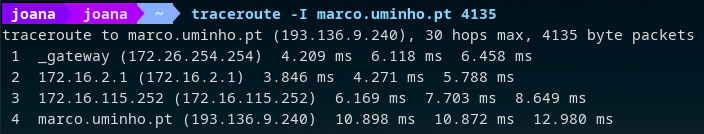
\includegraphics[width=400pt]{images/ParteI/Questao3/questao3-terminal.png}
    \caption{Resultado do comando \textit{traceroute} com tamanho de pacote definido.} \label{questao3-terminal}
    \end{figure}
    


\subsubsection{Localize a primeira mensagem ICMP. Porque é que houve necessidade de fragmentar o pacote inicial?}

    \begin{figure}[H]
    \centering
    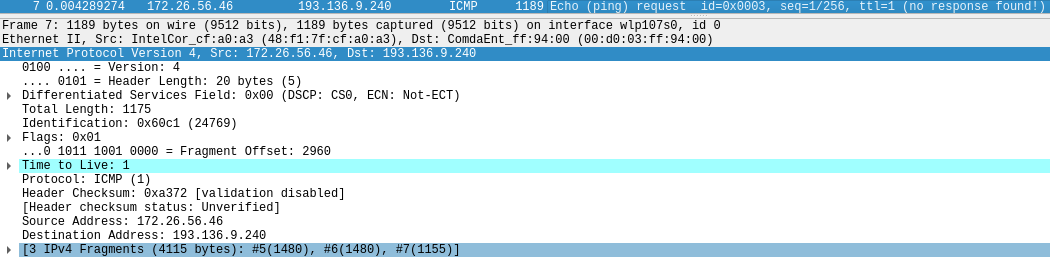
\includegraphics[width=500pt]{images/ParteI/Questao3/questao3-UltimoSegmento.png}
    \caption{Primeiro pacote ICMP enviado pela máquina.} \label{questao3-ICMP}
    \end{figure}
    
    \par Foi necessário fragmentar o primeiro pacote visto que o limite da camada de \textit{IP} é de 1500 \textit{bytes} em contraste com o tamanho do pacote a ser enviado (4135 \textit{bytes}), ou seja o MTU é inferior ao tamanho do pacote a ser enviado.

\subsubsection{Imprima o primeiro fragmento do datagrama IP segmentado. Que informação no cabeçalho indica que o datagrama foi fragmentado? Que informação no cabeçalho IP indica que se trata do primeiro fragmento? Qual é o tamanho deste datagrama IP?}

    \begin{figure}[H]
    \centering
    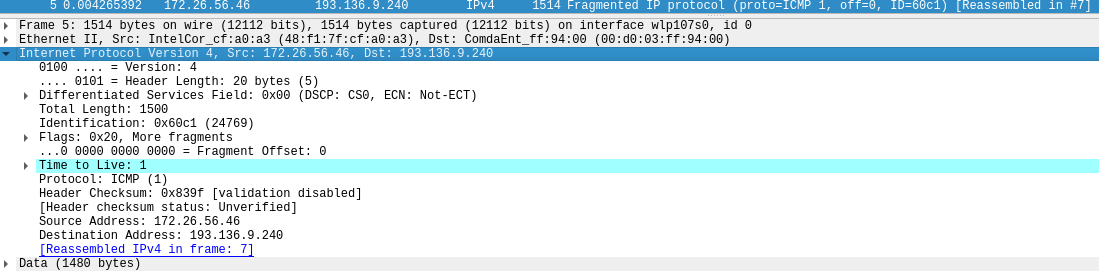
\includegraphics[width=500pt]{images/ParteI/Questao3/questao3-firstSegmentado.png}
    \caption{Primeiro pacote fragmentado.} \label{questao3-primeiroSeg}
    \end{figure}
    
    \par O cabeçalho indica-nos que o datagrama foi fragmentado pois tem a \textit{flag \textbf{More Fragments}} acionada. Para além disto, sabemos que se trata do primeiro fragmento do datagrama original pois o valor no campo \textit{\textbf{Fragment Offset}} é 0, ou seja, este datagrama tem um deslocamento de dados igual a 0 relativamente ao datagrama original. Assim, este datagrama tem um tamanho de 1500 \textit{bytes} (20 para cabeçalho e 1480 para dados).
    
    
\subsubsection{Imprima o segundo fragmento do datagrama IP original. Que informação do cabeçalho IP indica que não se trata do 1º fragmento? Há mais fragmentos? O que nos permite afirmar isso?}

    \begin{figure}[H]
    \centering
    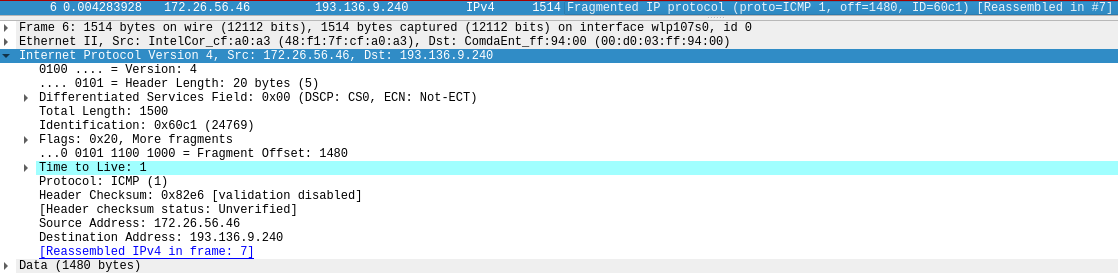
\includegraphics[width=500pt]{images/ParteI/Questao3/questao3-secondSegment.png}
    \caption{Segundo pacote fragmentado.} \label{questao3-segundoSeg}
    \end{figure}
    
    \par Conseguimos verificar, através do valor presente no campo \textit{\textbf{Fragment Offset}} do cabeçalho, que não se trata do primeiro fragmento do datagrama, uma vez que esse valor é diferente de 0, sendo, neste caso, 1480, indicando, por isso, um deslocamento de 1480 \textit{bytes} relativamente ao datagrama original. Para além disto, conseguimos denotar que se vão seguir mais fragmentos através do acionamento da \textit{flag \textbf{More Fragments}}.
    
\subsubsection{Quantos fragmentos foram criados a partir do datagrama original?}

    \par A partir do datagrama original, foram criados três fragmentos como podemos ver pelas Figuras acima. O primeiro fragmento (Figura \ref{questao3-primeiroSeg}) e o segundo (Figura \ref{questao3-segundoSeg}) com um total de 1480 \textit{bytes} de dados. Por fim, o último fragmento (Figura \ref{questao3-ICMP}) corresponde ao primeiro pacote ICMP enviado pela máquina, com um total de 1155 \textit{bytes} de dados.
    
    
\subsubsection{Indique, resumindo, os campos que mudam no cabeçalho IP entre os diferentes fragmentos, e explique a forma como essa informação permite reconstruir o datagrama original.}

    \par Os campos que se vão alterando ao longo da sequência de fragmentos são \textit{checksum}, \textit{flags}, \textit{offset} e o tamanho do último fragmento relativamente aos anteriores, uma vez que apenas este pode ter ou não o número máximo de dados por pacote. O valor de \textit{checksum}, como referido em alíneas anteriores, serve para verificar a integridade do pacote, no entanto, não tem relação direta com a reconstrução do datagrama original. Já os campos das \textit{flags} e o \textit{offset} permitem fazer a reconstrução do datagrama, na medida em que o \textit{offset} indica a posição do fragmento relativamente aos dados originais, permitindo a ordenação correta dos fragmentos, e as \textit{flags} permitem afirmar se estamos localizados no último pacote ou se ainda existem mais.
    
    
\subsubsection{Verifique o processo de fragmentação através de um processo de cálculo.}

    \begin{figure}[H]
    \centering
    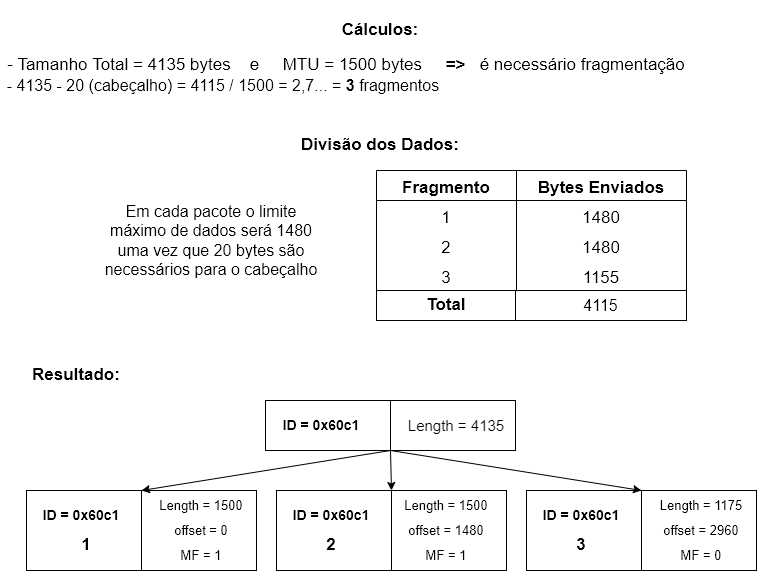
\includegraphics[width=490pt]{images/ParteI/Questao3/fragmentacao.png}
    \label{questao3-Calculo}
    \end{figure}
    
    \vspace{0.5cm}
    \par Como podemos verificar pelos cálculos, o datagrama original teria de ser dividido em três fragmentos. Os fragmentos mantêm o mesmo campo de identificação do datagrama original, alterando apenas as \textit{flags} de \textit{More Fragments} (MF) e o valor do \textit{offset} relativamente ao original. A \textit{flag} MF está apresentada com os valores 0 (equivalente ao valor '\textit{not set}') e 1, tendo estes o significado de não acionada e acionada, respetivamente.
    
    \par De forma adicional, podemos reparar que o \textit{overhead} de cabeçalho aumentou, uma vez que originalmente tínhamos apenas 20 \textit{bytes} de cabeçalho e devido à fragmentação obtivemos um conjunto de três cabeçalhos, ou seja, 60 \textit{bytes}.  
    Como consequência, houve um aumento do número total de \textit{bytes} transferidos na rede, pois no datagrama original seriam 4135 \textit{bytes} em contraste com a fragmentação, onde se registaram no total: 4115 (dados) + 3 * 20 (cabeçalho) = 4175 \textit{bytes}.
    
    \par Em suma, todos os valores calculados coincidiram com os valores presentes nos campos dos datagramas fragmentados capturados pelo programa.
    
    
\newpage
\subsubsection{Escreva uma expressão lógica que permita detetar o último fragmento correspondente ao datagrama original.}

    \par De acordo com os parâmetros do cabeçalho dos pacotes analisados nas alíneas acima, conseguimos deduzir os campos que afetam diretamente a deteção do último fragmento da \textit{stream}, sendo estes a \textit{flag more fragments} e o campo \textit{offset}. O valor do campo \textit{offset} tem de ser diferente de zero para assim concluirmos que, antes de mais, se trata de um datagrama fragmentado. A \textit{flag more fragments} transmite a informação se o fragmento se trata do último ou não. Por último, para o pacote fragmentado corresponder a um fragmento do original que procuramos, o campo de identificação tem de ser igual. Assim, apresentamos a expressão lógica capaz de detetar o último fragmento tendo em conta estes campos do cabeçalho:

    \paragraph{}
    \begin{minipage}{\linewidth}
        \centering
        \fbox{
        ID == original \space\space \&\& \space\space More Fragments == \textit{not set} \space\space \&\& \space\space offset \begin{math}  > 0 \end{math}
        }
    \end{minipage}
    
    \paragraph{}
    \par De seguida, de forma a testar a nossa expressão, executamos a mesma na secção de \textit{filter} da ferramenta \textit{Wireshark} com a única diferença de não incluirmos a verificação do campo de identificação, obtendo assim todos os últimos fragmentos de todos os datagramas que sofreram fragmentação. Como podemos conferir pela Figura \ref{questao3-ultima}, obtivemos o resultado esperado:
    
    \begin{figure}[H]
    \centering
    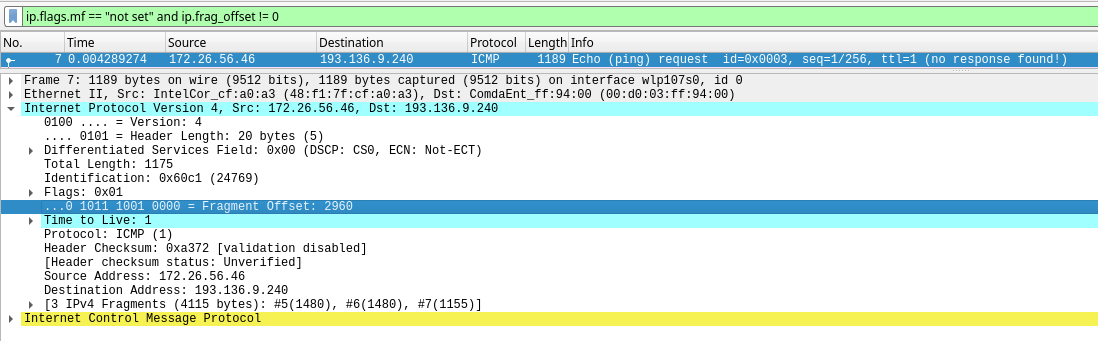
\includegraphics[width=490pt]{images/ParteI/Questao3/questao3-ultima.png}
    \caption{Verificação da expressão na ferramenta \textit{Wireshark}.}
    \label{questao3-ultima}
    \end{figure}

% ----- PARTE II ------
% -------------------------------------- PARTE II -------------------------------------


\newpage
\section*{\hfil Parte II\hfil}

\section{Questões e Respostas}

\subsection{Questão 1 - Topologia LEI-RC}
\subsubsection{Indique que endereços IP e máscaras de rede foram atribuídos pelo CORE a cada equipamento. Para simplificar, pode incluir uma imagem que ilustre de forma clara a topologia definida e o endereçamento usado.}

    Pela Figura \ref{parteII-questao1-topologia} conseguimos ter uma visão geral da topologia assim como a divisão entre os vários departamentos. Assim, a todos os endereços é aplicada uma máscara de rede de 25  \textit{bits}, sendo os endereços das sub-redes dos departamentos os seguintes: 

    \begin{multicols}{2}
    \begin{itemize}
        \item \textbf{Departamento A:} 10.0.4.0 
        \item \textbf{Departamento B:} 10.0.5.0 
        \item \textbf{Departamento C:} 10.0.6.0 
        \item \textbf{Departamento D:} 10.0.7.0 
    \end{itemize}
    \end{multicols}


    \begin{figure}[H]
    \centering
    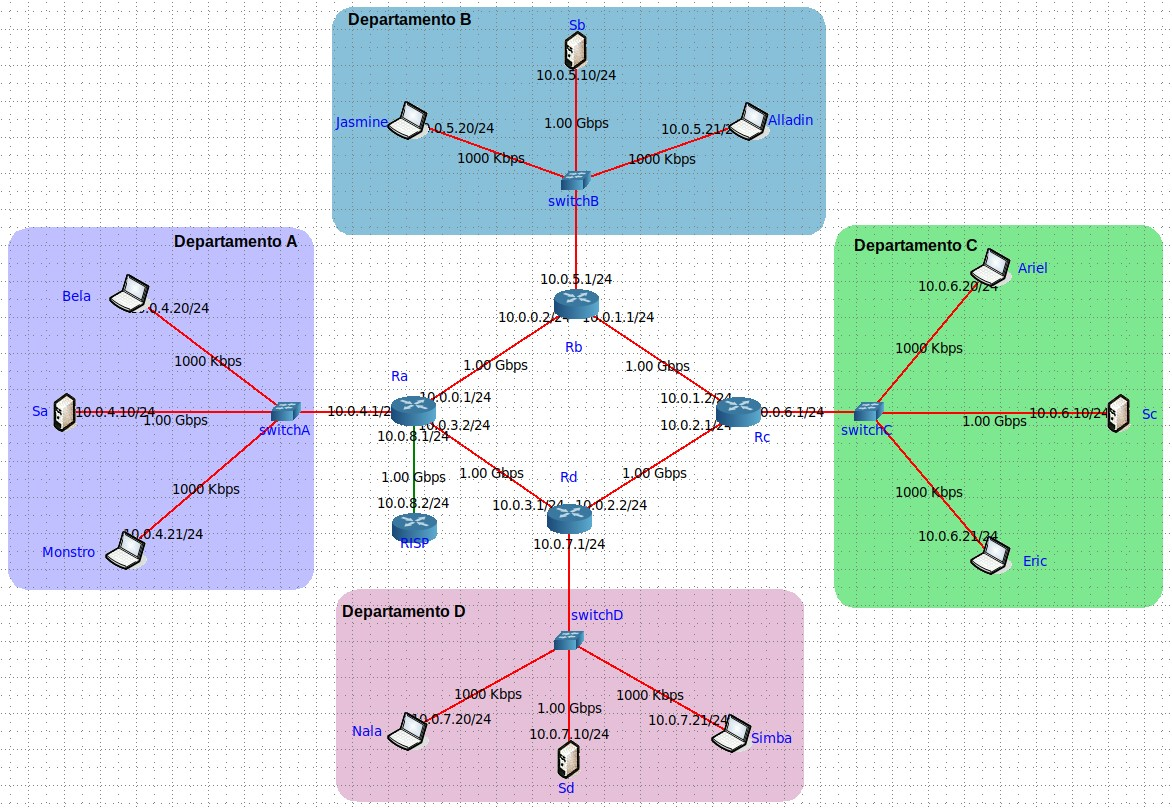
\includegraphics[width=500pt]{images/ParteII/Questao1/TopologiaOriginal.jpg}
    \caption{Topologia LEI-RC.} \label{parteII-questao1-topologia}
    \end{figure}
    
    
    

\subsubsection{Tratam-se de endereços privados? Porquê?}
    
    \par Geralmente os endereços privados encontram-se reservados entre intervalos específicos geridos pela \textit{Internet Assigned Numbers Authority (IANA)} e, por essa razão, não podem ser atribuídos de forma arbitrária. Apresentamos, então, alguns intervalos reservados para endereços privados: 
    
        \begin{itemize}
            \item 10.0.0.0 - 10.255.255.255 / 8
            \item 172.16.0.0 - 172.31.255.255 / 12
            \item 192.168.0.0 - 192.168.255.255 / 16
        \end{itemize}
        
        \par Visto que todos os endereços presentes na topologia se encontram incluídos no intervalo de endereços do primeiro ponto, podemos afirmar que os endereços se tratam de endereços privados.
        
        
        
        
    
\subsubsection{Porque razão não é atribuido um endereço IP aos switches?}

    \par Os \textit{switches} tratam-se de dispositivos que simplesmente conectam todos os elementos da rede. Estes atuam como ponte ou unidade de controlo para que os dispositivos possam comunicar entre si.
    Estes pertencem à camada dois do modelo de referência OSI, ou seja, camada de \textit{Link}. Esta camada está localizada diretamente abaixo da camada de rede (camada três) que funciona sobre endereços IP, no entanto, a camada de \textit{Link} utiliza endereços MAC (endereços físicos) daí não ter sido atribuído endereço IP aos \textit{switches}.  
    
    
    
    
    
\subsubsection{Usando o comando \textit{\textbf{ping}} certifique-se que existe conectividade IP interna a cada departamento (e.g. entre um laptop e o servidor respetivo).}

    \par Como podemos ver pelas figuras apresentadas abaixo, existe conectividade interna nos vários departamentos uma vez que existe resposta (\textit{echo reply}) ao envio de pacotes (\textit{echo request}) entre dispositivos no mesmo departamento.
    
    \begin{minipage}{0.5\linewidth}
    \centering
        \begin{figure}[H]
        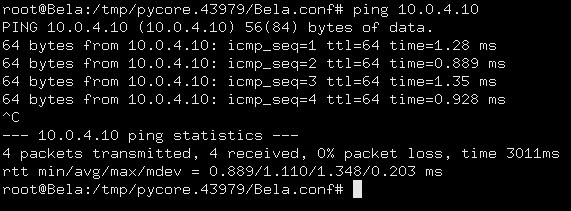
\includegraphics[width=\linewidth]{images/ParteII/Questao1/parteII-questao1-d-Bela.jpg}
        \caption{Departamento A (Bela - Sa).} \label{parteII-questao1-ping-Bela-SA}
        \end{figure}
    \end{minipage}
    \begin{minipage}{0.5\linewidth}
    \centering
        \begin{figure}[H]
        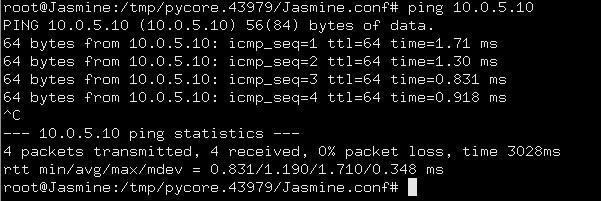
\includegraphics[width=\linewidth]{images/ParteII/Questao1/parteII-questao1-d-Jasmine.jpg}
        \caption{Departamento B (Jasmine -Sb).} \label{parteII-questao1-ping-Jamsmine-SB}
        \end{figure}
    \end{minipage}
    
    \begin{minipage}{0.5\linewidth}
    \centering
         \begin{figure}[H]
        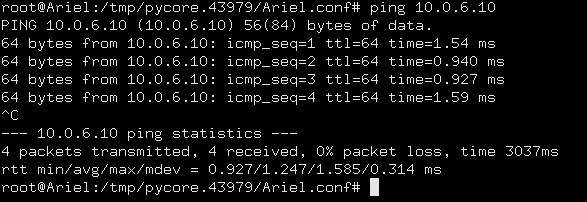
\includegraphics[width=\linewidth]{images/ParteII/Questao1/parteII-questao1-d-Ariel.jpg}
        \caption{Departamento C (Ariel - Sc).} \label{parteII-questao1-ping-Ariel-SC}
        \end{figure}
    \end{minipage}
    \begin{minipage}{0.5\linewidth}
    \centering
        \begin{figure}[H]
        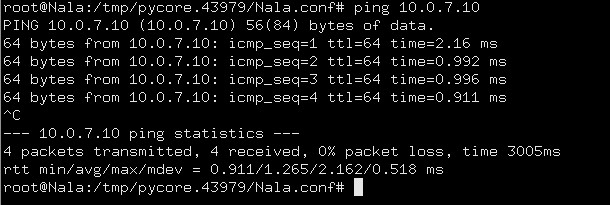
\includegraphics[width=\linewidth]{images/ParteII/Questao1/parteII-questao1-d-Nala.jpg}
        \caption{Departamento D (Nala - Sd).} \label{parteII-questao1-ping-Nala-SD}
        \end{figure}    
    \end{minipage}
    
    
    
    
    
    
\subsubsection{Execute o número mínimo de comandos \textit{\textbf{ping}} que lhe permite verificar a existência de conectividade IP entre departamentos.}

    \par Para verificar a conectividade IP entre os vários departamentos, apenas executamos o comando \textit{ping} duas vezes, sendo estas: 
    
        \begin{itemize}
            \item Departamento A $\xrightarrow[]{}$ Departamento C (Figura \ref{parteII-questao1-ping-A-C})
            
            \item Departamento D $\xrightarrow[]{}$ Departamento B (Figura \ref{parteII-questao1-ping-D-B})
        \end{itemize}
    
    \par Uma vez que o \textit{ping} do departamento A para o C garante que o tráfego na direção horizontal da topologia está a ser encaminhado corretamente e o \textit{ping} do departamento D ao B garante o bom encaminhamento vertical do tráfego da topologia, conseguimos, assim, garantir a conectividade entre todos os departamentos pois temos garantias do correto funcionamento dos quatro \textit{routers}.
    
    \begin{minipage}{0.5\linewidth}
    \centering
        \begin{figure}[H]
        \centering
        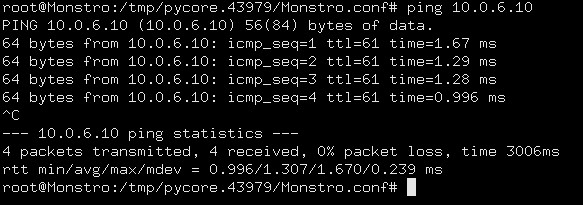
\includegraphics[width=\linewidth]{images/ParteII/Questao1/parteII-questao1-e-A-C.jpg}
        \caption{Ping do Departamento A para o C.} \label{parteII-questao1-ping-A-C}
        \end{figure}
    \end{minipage}
    \begin{minipage}{0.5\linewidth}
    \centering
        \begin{figure}[H]
        \centering
        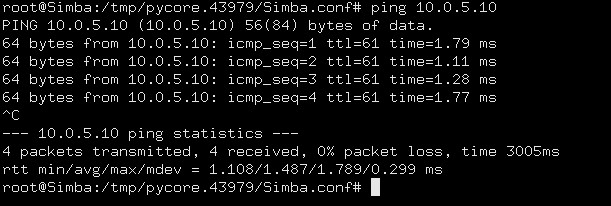
\includegraphics[width=\linewidth]{images/ParteII/Questao1/parteII-questao1-e-D-B.jpg}
        \caption{Ping do Departamento D para o B.} \label{parteII-questao1-ping-D-B}
        \end{figure}
    \end{minipage}
    
    
    
    
\paragraph{}
\subsubsection{Verifique se existe conectividade IP do portátil Bela para o router de acesso Risp.}

    \par Como podemos verificar pela Figura \ref{parteII-questao1-f-BelaISP}, ao executar o comando \textit{ping} do portátil Bela para o \textit{router} de acesso Risp, este obtém resposta provando assim a conectividade entre os mesmos.
    
    \textbf{\begin{figure}[H]
    \centering
    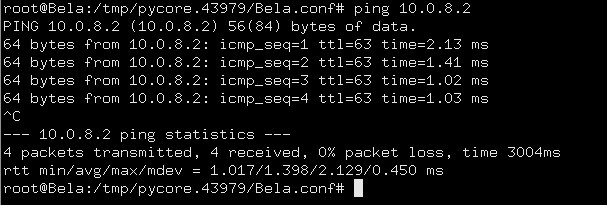
\includegraphics[width=300pt]{images/ParteII/Questao1/parteII-questao1-f-BelaISP.jpg}
    \caption{Ping Bela - Risp} \label{parteII-questao1-f-BelaISP}
    \end{figure}}














\newpage
\subsection{Questão 2 - Tabelas de Encaminhamento (Bela - Ra)}

\subsubsection{Execute o comando \textit{\textbf{netstat -rn}} por forma a poder consultar a tabela de encaminhamento unicast (IPV4). Interprete as várias entradas de cada tabela}
    
    \begin{figure}[H]
    \centering
    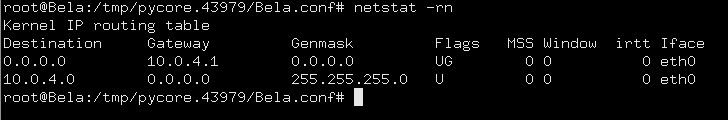
\includegraphics[width=450pt]{images/ParteII/Questao2/parteII-questao2-a-Bela.jpg}
    \caption{Tabela de Encaminhamento do \textit{host} Bela.} \label{parteII-questao2-a-tabelaBela}
    \end{figure} 
    
    \begin{figure}[H]
    \centering
    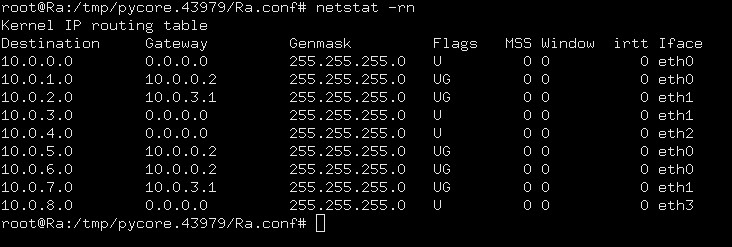
\includegraphics[width=450pt]{images/ParteII/Questao2/parteII-questao2-a-RA.jpg}
    \caption{Tabela de Encaminhamento do \textit{router} Ra.} \label{parteII-questao2-a-tabelaRa}
    \end{figure} 
        
    \par Uma tabela de encaminhamento fornece instruções para determinar o próximo salto de um pacote de dados numa rede IP. Como tal, tem de possuir parâmetros que permitam executar esse mesmo encaminhamento. Assim, apresentamos, também em formato tabela, a descrição das várias colunas da tabela de encaminhamento dos dois dispositivos:
    
    \begin{center}
        \begin{tabular}{|c|c|}
        \hline
            \cline{1-2}
            Coluna & Descrição  \\
            \hline \hline
            Destination & endereço IP de rede destino \\
            Gateway & endereço IP do próximo salto \\
            Genmask & máscara a aplicar à coluna Destination \\
            Flags* & informação sobre a rota \\
            MSS & tamanho máximo de segmentos TCP \\
            Window & tamanho \textit{default} da janela TCP \\
            irtt & RTT estimado (inicial) \\
            Iface & interface de saída \\
            \cline{1-2}
        \end{tabular}
    \end{center}
    
    \par * Existem várias \textit{flags} disponíveis, no entanto, nas figuras acima, apenas percepcionamos a \textbf{U} e \textbf{G}. A presença da \textit{flag} U determina que a rota está disponível e a \textit{flag} G indica a utilização da \textit{Gateway}.
    
    \newpage
    \par Relativamente às entradas das duas tabelas de encaminhamento, estas possuem a informação necessária para os pacotes de dados enviados por estes conseguirem alcançar o seu destino. 
    
    \par Em concreto, o portátil Bela apenas possui duas entradas que por sua vez descrevem a única interface de saída do mesmo, estando a primeira definida como rota por defeito e a segunda como próximo salto caso o destino seja a sua própria rede. Assim, o portátil Bela consegue assegurar o tráfego dos seus pacotes uma vez que, por defeito, redireciona o tráfego para o \textit{router} Ra.
    
    \par O \textit{router} Ra possui entradas para todas as sub-redes presentes na topologia, permitindo assim encaminhar tráfego para as mesmas. Para além disto, conseguimos denotar que todas as entradas com endereço IP 0.0.0.0 na coluna \textit{Gateway} têm como destino uma sub-rede da qual o \textit{router} já faz parte, isto acontece porque uma vez que o \textit{router} já está integrado na sub-rede, então já não existe \textit{gateway}.
    
    
    

\paragraph{}
\subsubsection{Diga, justificando, se está a ser usado encaminhamento estático ou dinâmico}

    \begin{figure}[H]
    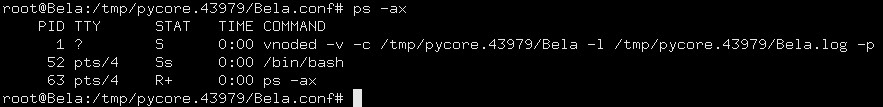
\includegraphics[width=\linewidth]{images/ParteII/Questao2/parteII-questao2-b-Bela.jpg}
    \caption{Resultado do comando no \textit{host} Bela.} \label{parteII-questao2-b-encaminhamentoBela}
    \end{figure} 
    
    \begin{figure}[H]
    \centering
    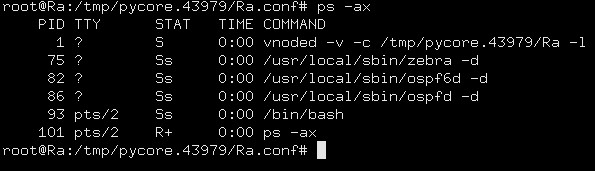
\includegraphics[width=400pt]{images/ParteII/Questao2/parteII-questao2-b-RA.jpg}
    \caption{Resultado do comando no \textit{router} RA.} \label{parteII-questao2-b-encaminhamentoRA}
    \end{figure} 
    
    
    \par Pelas Figuras \ref{parteII-questao2-b-encaminhamentoBela} e \ref{parteII-questao2-b-encaminhamentoRA} conseguimos perceber algumas diferenças nos processos que estão a decorrer em cada um dos dispositivos. A presença de um processo que termina com \textit{\textbf{ospf}} significa que o protocoloo OSPF está a ser utilizado. O protocolo OSPF (\textit{Open Shortest Path First}), é um protocolo de descoberta de vizinhos, isto é, os \textit{routers} ou \textit{hosts} depois de garantirem que as suas interfaces estão funcionais, enviam pacotes '\textit{Hello}' para descobrir os dispositivos adjacentes (vizinhos) e as rotas conhecidas pelos mesmos. A utilização do protocolo OSPF garante um encaminhamento dinâmico, uma vez que este, através da comunicação entre os vários dispositivos, define o melhor caminho.
    Assim, podemos concluir que o portátil Bela não utiliza encaminhamento dinâmico, contrariamente ao \textit{router} Ra que utiliza.
    
    
    
    
    
\subsubsection{Admita que, por questões administrativas, a rota por defeito (\textit{\textbf{0.0.0.0}} ou \textit{\textbf{default}}) deve ser retirada definitivamente da tabela de encaminhamento do servidor Sa. Use o comando \textit{\textbf{route delete}} para o efeito. Que implicações tem esta medida para os utilizadores da LEI-RC que acedem ao servidor. Justifique.}
    
    \paragraph{}
    \paragraph{}
    \begin{figure}[H]
    \centering
    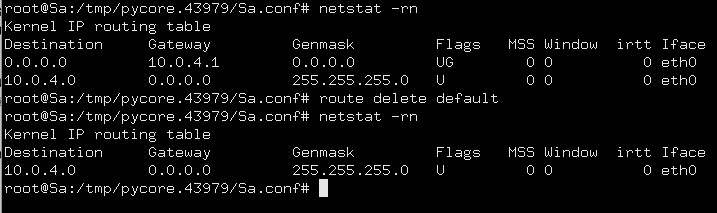
\includegraphics[width=400pt]{images/ParteII/Questao2/parteII-questao2-c-SA-delete.jpg}
    \caption{Comando \textit{route delete} executado.} \label{parteII-questao2-c-deleteSA}
    \end{figure} 
    

    \par Pela Figura \ref{parteII-questao2-c-deleteSA} conseguimos perceber que após retirada da rota por defeito da tabela de encaminhamento do servidor Sa, este apenas possui a entrada para o encaminhamento de dados que tenham como destino a sua própria sub-rede. Em consequência, e sabendo que a rota por defeito é a rota a seguir caso não exista uma entrada específica na tabela de encaminhamento para a rede destino requerida, ao retirarmos esta mesma entrada, estamos a impossibilitar a comunicação do servidor com dispositivos que se encontrem fora da sua sub-rede (10.0.4.0), pois este apesar de conseguir receber dados não irá conseguir responder. Assim, apresentamos de seguida o comando \textit{ping} com origem num \textit{host} de outra sub-rede (servidor Sc), provando que o servidor Sa não consegue comunicar de volta, pois a percentagem de pacotes perdidos (\textit{packet loss}) é de 100\%:
    
    \paragraph{}
    \begin{figure}[H]
    \centering
    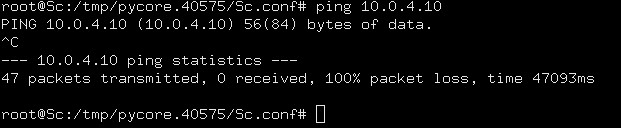
\includegraphics[width=400pt]{images/ParteII/Questao2/questao2-pingSAdeleted.jpg}
    \caption{Comando \textit{ping} ao servidor Sa.} \label{parteII-questao2-Sc-Sa-deleteSA-ping}
    \end{figure} 
    
    
    
\subsubsection{Não volte a repor a rota por defeito. Adicione todas as rotas estáticas necessárias para restaurar a conectividade para o servidor Sa, por forma a contornar a restrição imposta na alínea c). Utilize para o efeito o comando \textit{\textbf{route add}} e registe os comandos que usou.}
    
    \begin{figure}[H]
    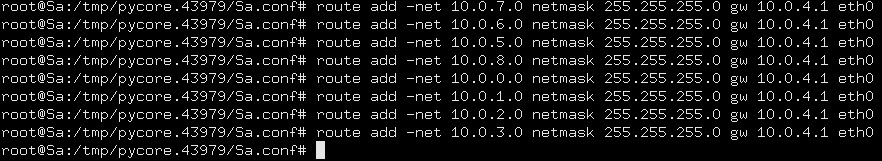
\includegraphics[width=\linewidth]{images/ParteII/Questao2/parteII-questao2-d-SA-ADD.jpg}
    \caption{Comandos utilizados para adicionar as rotas à tabela de encaminhamento.} \label{parteII-questao2-d-novoTabelaSA}
    \end{figure} 
    
    
    \par Como podemos ver pela Figura \ref{parteII-questao2-d-novoTabelaSA}, foram adicionadas estaticamente todas as sub-redes presentes na topologia LEI-RC utilizando como \textit{gateway} o endereço IP do \textit{router} Ra que anteriormente estava definida como rota por defeito, permitindo restaurar a conectividade para o servidor Sa.
    
    
    
    
\paragraph{}
\subsubsection{Teste a nova política de encaminhamento garantindo que o servidor está novamente acessível, utilizando para o efeito o comando \textit{\textbf{ping}}. Registe a nova tabela de encaminhamento do servidor.}
  
    \begin{figure}[H]
    \centering
    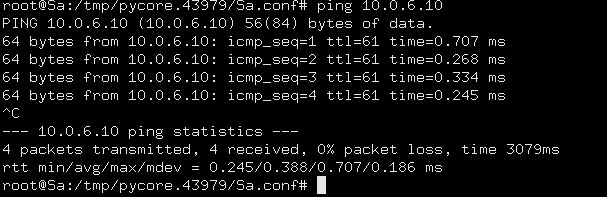
\includegraphics[width=400pt]{images/ParteII/Questao2/parteII-questao2-e-SA-PING.jpg}
    \caption{Comando \textit{ping} do servidor Sa para o servidor Sc.} \label{parteII-questao2-e-PING}
    \end{figure} 
    
    
    \par Pela Figura \ref{parteII-questao2-e-PING}, conseguimos denotar que o servidor está novamente acessível, uma vez que utilizamos o comando \textit{ping} com destino no servidor Sc, estando este presente numa sub-rede diferente da do servidor Sa, provando assim que o servidor consegue novamente comunicar com os dispositivos localizados fora da sua sub-rede. 

    \paragraph{}
    \begin{figure}[H]
    \centering
    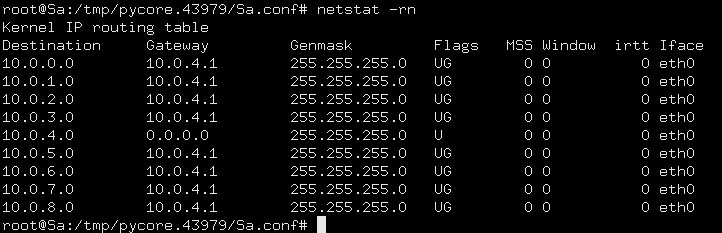
\includegraphics[width=400pt]{images/ParteII/Questao2/parteII-questao2-e-SA-TABELA.jpg}
    \caption{Tabela de Encaminhamento do servidor Sa.} \label{parteII-questao2-e-TABELA}
    \end{figure} 
  
  
    \par De seguida, consultamos a nova tabela de encaminhamento do servidor (Figura \ref{parteII-questao2-e-TABELA}), denotando as entradas que substituíram a rota por defeito, ou seja, entradas de todas as sub-redes da topologia. Adicionalmente, é de notar que a rota por defeito tem como objetivo, entre outros, reduzir a tabela de encaminhamento, agregando todas as rotas que possuem como endereço IP destino sub-redes exteriores, neste caso, ao servidor. Assim, o crescimento da tabela de encaminhamento após retirada da rota por defeito é notório como podemos comprovar pela comparação das Figuras \ref{parteII-questao2-c-deleteSA} (após retirada da rota por defeito) e \ref{parteII-questao2-e-TABELA} (após introdução estática das rotas).
  
  
  
  
  
  
  
  
  
  
  
  
  
\newpage  
\subsection{Questão 3 -  Definição de Sub-redes}

\subsubsection{Considere que dispõe apenas do endereço da rede IP 192.168.XXX.128/25, em que XXX é o decimal correspondendo ao seu número de grupo (PLXXX). Defina um novo esquema de endereçamento para as redes dos departamentos (mantendo as redes de acesso externo e \textit{backbone} inalteradas), sabendo que o número de departamentos pode vir a aumentar no curto prazo. Atribua endereços às interfaces dos vários sistemas envolvidos. Assuma que todos os endereços de sub-redes são usáveis.}

    \par 
    
    \begin{figure}[H]
    \centering
    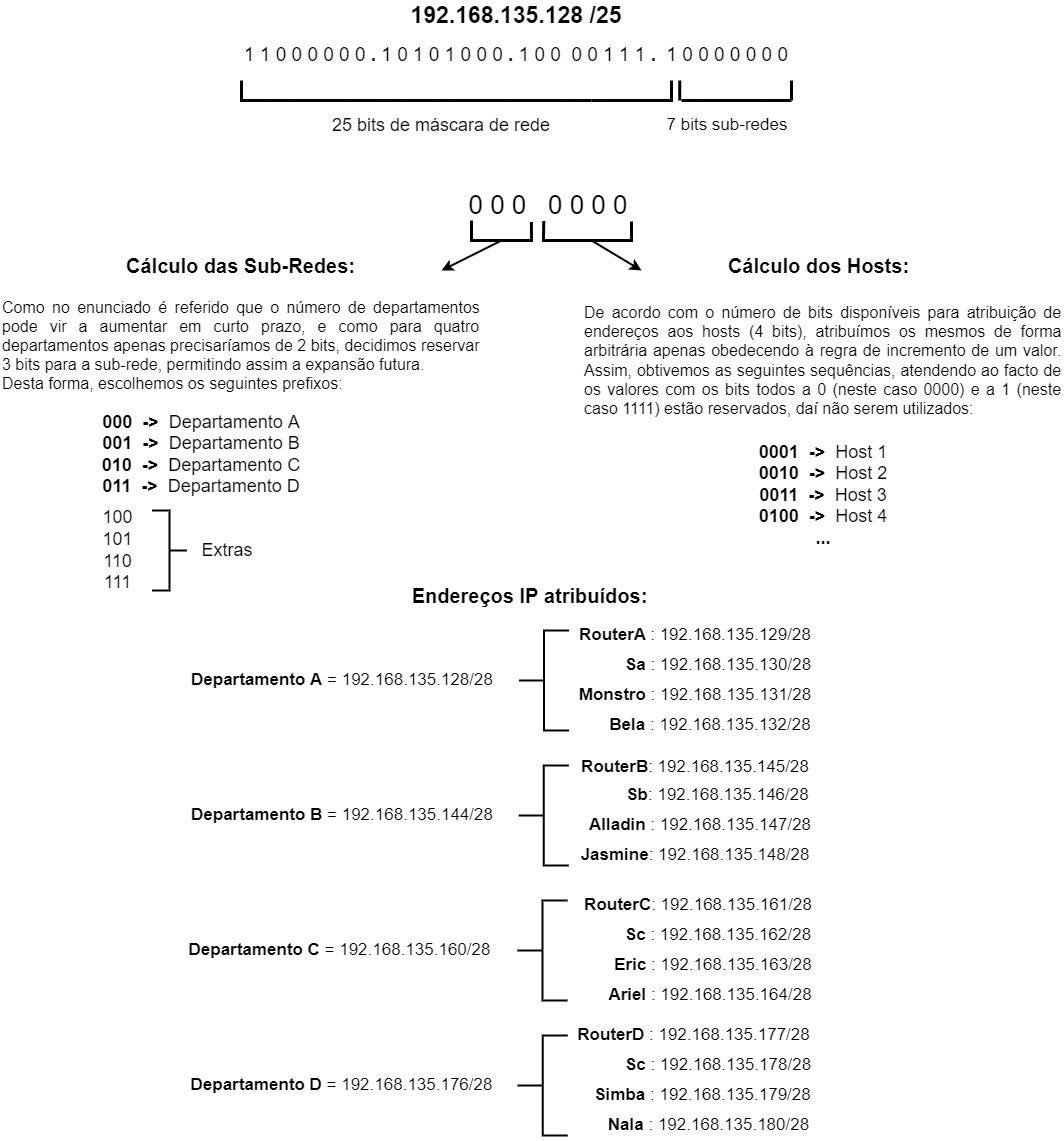
\includegraphics[width=500pt]{images/ParteII/Questao3/Questao3-ParteII-RC-Questao3.drawio.png}
    \label{parteII-questao3-subnetting}
    \end{figure}
    
    \par \textbf{NOTA:} Por simplificação, na figura apresentada de seguida, os endereços IP das interfaces de ligação dos \textit{routers} não estão presentes, mas é subentendida a sua presença. Assim, apresentamos uma vista simplificada da topologia com as diversas sub-redes (Departamentos):
    \paragraph{}
    \begin{figure}[H]
    \centering
    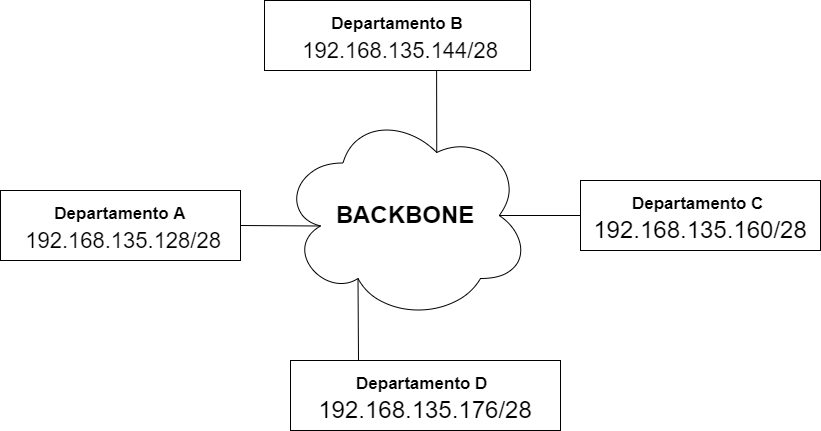
\includegraphics[width=450pt]{images/ParteII/Questao3/Questao3-Topologia.png}
    \caption{Vista simplificada da rede após aplicação de \textit{Subnetting}.}
    \label{parteII-questao3-topologia}
    \end{figure}
    
    %\par Os endereços dos routers ficaram com o primeiro endereço de forma aleatória, podendo estes possuir qualquer valor de endereço no intervalo determinado para a sub-rede.
    
    
    
\paragraph{}    
\subsubsection{Qual a máscara de rede que usou (em formato decimal)? Quantos \textit{hosts} IP pode interligar em cada departamento? Quantos prefixos de sub-rede ficam disponíveis para uso futuro? Justifique.}

    \par A máscara de rede utilizada foi de /28 \textit{bits} (255.255.255.240) uma vez que foram utilizados mais 3 \textit{bits} para representar as diversas sub-redes. Assim, em cada departamento é possível interligar no máximo 14 \textit{hosts} uma vez que todos têm disponíveis para o efeito 4 \textit{bits} (2\textsuperscript{4} - 2). Relativamente aos prefixos de sub-rede disponíveis para uso futuro, sobraram 4 prefixos possíveis, pois, uma vez que foram utilizados 3 \textit{bits} para atribuição de sub-redes, há um total de oito combinações tendo quatro destas sido já atribuídas aos vários departamentos. Assim, sobraram os seguintes prefixos: 100, 101, 110 e 111.
    
    
    

\newpage
\subsubsection{Verifique e garanta que a conectividade IP interna na rede local LEI-RC é mantida. No caso de não existência de conectividade, reveja a atribuição de endereços efetuada e eventuais erros de encaminhamento por forma a realizar as correções necessárias. Explique como procedeu.}

    \paragraph{}
    \paragraph{}
    \begin{figure}[H]
    \centering
    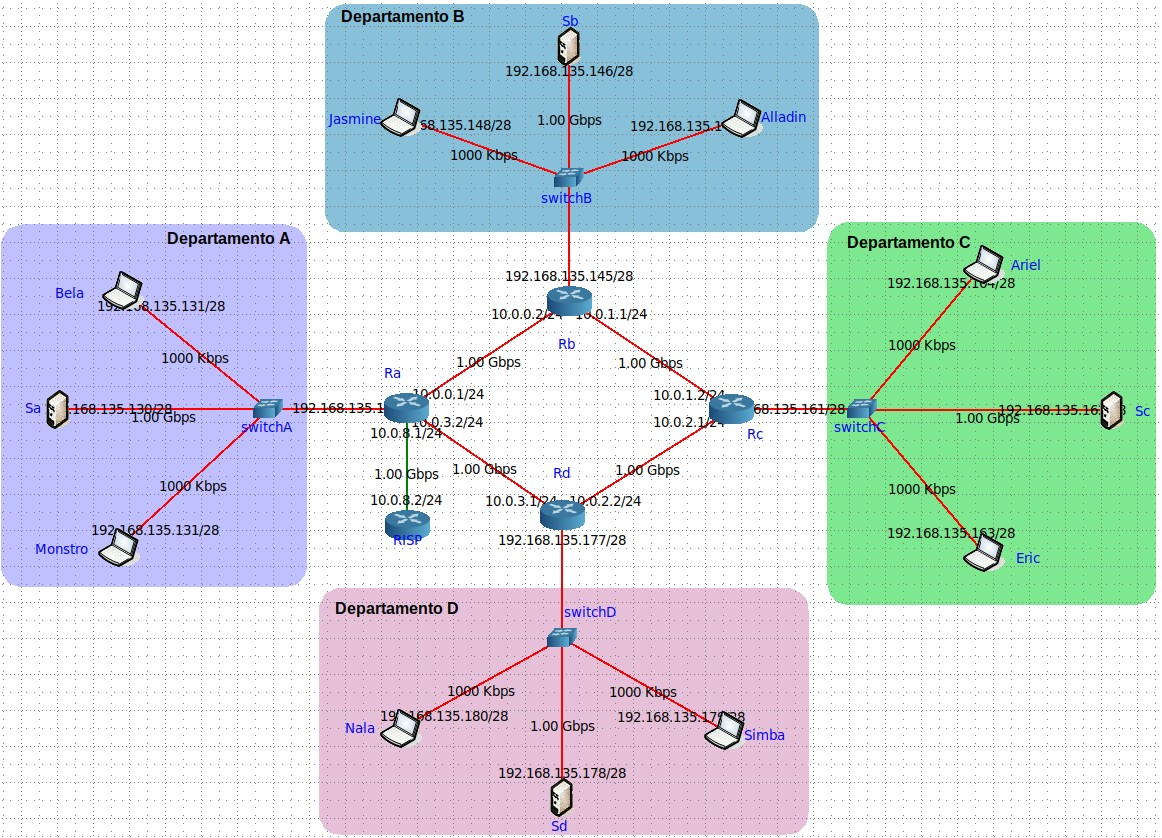
\includegraphics[width=500pt]{images/ParteII/Questao3/TopoSubnetting.jpg}
    \label{parteII-questao3-subnettingNovo}
    \caption{Topologia após aplicação de \textit{Subnetting}.}
    \end{figure}
    
    
    \paragraph{}
    \par Depois da modificação da topologia para a inclusão dos endereços obtidos por \textit{subnetting}, de forma a testar a conectividade na topologia LEI-RC, seguimos o método utilizado na questão 1 da parte II presente neste mesmo relatório, isto é, começamos por verificar a \textbf{conectividade interna} nos vários departamentos, terminando na verificação da \textbf{conectividade inter-departamentos}. Assim, apresentamos a sequência de comandos \textit{ping} utilizados para o efeito:
    
    
    \begin{minipage}{0.5\linewidth}
    \centering
        \begin{figure}[H]
        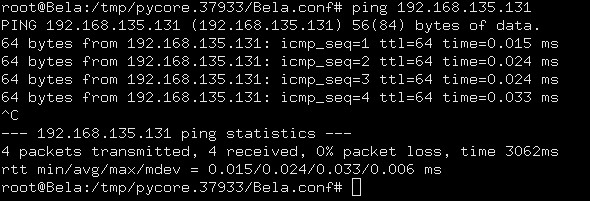
\includegraphics[width=\linewidth]{images/ParteII/Questao3/questao3-DepA-Bela-Monstro.jpg}
        \caption{Departamento A (Bela - Monstro).} \label{parteII-questao3-ping-Bela-Monstro}
        \end{figure}
    \end{minipage}
    \begin{minipage}{0.5\linewidth}
    \centering
        \begin{figure}[H]
        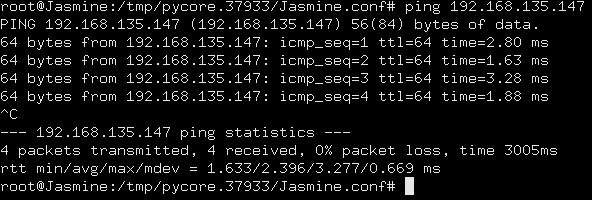
\includegraphics[width=\linewidth]{images/ParteII/Questao3/questao3-DepB-Jasmine-Alladin.jpg}
        \caption{Departamento B (Jasmine - Alladin).} \label{parteII-questao3-ping-Jamsmine-Alladin}
        \end{figure}
    \end{minipage}
    
    \begin{minipage}{0.5\linewidth}
    \centering
         \begin{figure}[H]
        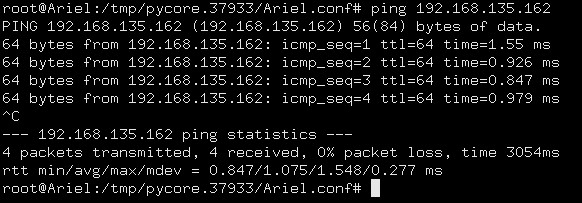
\includegraphics[width=\linewidth]{images/ParteII/Questao3/questao3-DepC-Ariel-Eric.jpg}
        \caption{Departamento C (Ariel - Eric).} \label{parteII-questao3-ping-Ariel-Eric}
        \end{figure}
    \end{minipage}
    \begin{minipage}{0.5\linewidth}
    \centering
        \begin{figure}[H]
        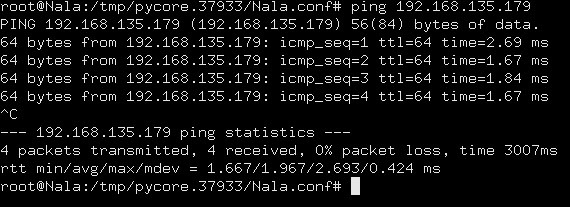
\includegraphics[width=\linewidth]{images/ParteII/Questao3/questao3-DepD-Nala-Simba.jpg}
        \caption{Departamento D (Nala - Simba).} \label{parteII-questao3-ping-Nala-Simba}
        \end{figure}    
    \end{minipage}
    
    
    \paragraph{}
    \begin{minipage}{0.5\linewidth}
    \centering
        \begin{figure}[H]
        \centering
        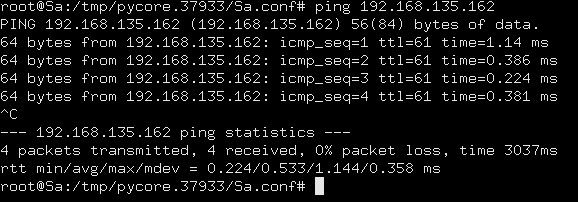
\includegraphics[width=\linewidth]{images/ParteII/Questao3/questao3-DepA-DepC-Sa-Sc.jpg}
        \caption{Ping do Departamento A para o C.} \label{parteII-questao3-ping-A-C}
        \end{figure}
    \end{minipage}
    \begin{minipage}{0.5\linewidth}
    \centering
        \begin{figure}[H]
        \centering
        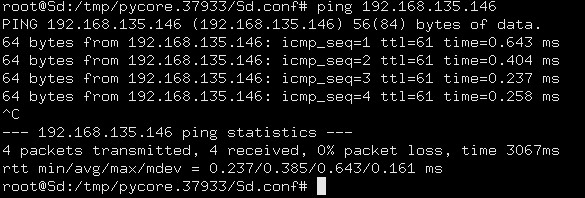
\includegraphics[width=\linewidth]{images/ParteII/Questao3/questao3-Depd-DepB-Sd-Sb.jpg}
        \caption{Ping do Departamento D para o B.} \label{parteII-questao3-ping-D-B}
        \end{figure}
    \end{minipage}


\newpage
\section{Conclusão}
    \par Com o finalizar deste trabalho, encontramo-nos, em geral, satisfeitos com o trabalho desenvolvido, tendo sido alcançados todos os objetivos propostos pelos docentes presentes nos enunciados da primeira e segunda partes que englobaram este segundo trabalho prático da unidade curricular.

    \par Na \textbf{primeira parte} deste trabalho, foi-nos proposto a resolução de vários exercícios e problemas da área de redes, nomeadamente o desenvolvimento de uma topologia, captura de pacotes através da ferramenta \textit{wireshark} e, por fim, a análise e manipulação de datagramas IP. Este desenvolvimento ocorreu sem grandes problemas estando o grupo bastante satisfeito com os resultados.
    
    \par Na \textbf{segunda parte}, especificamos ainda mais o objeto de estudo dos exercícios, focando-nos nas temáticas de endereçamento, encaminhamento e técnicas de \textit{subnetting}. Para além disto, foi necessário construir uma nova topologia que englobasse mais variáveis sendo, por isso, mais complexa que a desenvolvida anteriormente. Nesta parte conseguimos perceber que algumas alíneas poderiam ter sido resolvidas de maneira diferente, como, por exemplo, a alínea de inserção de novas rotas de forma estática no \textit{router} Ra após a remoção da rota por defeito. Esta poderia ter sido resolvida de forma mais eficiente utilizando a técnica de \textit{supernettting} diminuindo bastante o tamanho da tabela de encaminhamento do mesmo, no entanto, adicionamos entradas por cada sub-rede presente na topologia.
    
    \par Em suma, através deste projeto, conseguimos compreender a difícil e necessária organização dos vários componentes da rede e a importância de cada um destes para o bom funcionamento da mesma. Para além disto, a construção e desenvolvimento deste trabalho prático permitiu a todo o grupo aprofundar os seus conhecimentos, mesmo que introdutórios, na área de redes. Em consequência, depois deste trabalho atingimos uma ampla percepção de alguns assuntos da área como encaminhamento, endereçamento, \textit{subnetting} e fragmentação de datagramas.


\end{document}